%!TeX root=../thesis.tex
\tikzset{every picture/.style={line width=0.75pt}} % Set default line width to 0.75pt

\chapter{Implementation}

This section presents the implementation of the algorithm based on the work of \cite{Joos_2020}. For each step, we provide the corresponding pseudocode and demonstrate the correctness of the algorithm.

\section{Common Definitions}

Throughout this chapter, we use some abstract functions to streamline explanations. The total number of vertices is denoted by $n$, and the collection of graphs is represented by $G = \{G_1, G_2, \dots, G_n\}$, where each graph $G_i$ satisfies Dirac's condition.

\subsection{Structure of $edge(u, v, c)$}

Each edge in $G$ has three attributes:

\begin{itemize}
    \item $u$, $v$: vertices connected by the edge
    \item $c$: color of the edge, which also indicates that the edge belongs to graph $G_i$
\end{itemize}

\subsection{Function $check\_edge(G, u, v, c)$}

This function takes four parameters:

\begin{itemize}
    \item $G$: the collection of graphs
    \item $u$: a vertex
    \item $v$: a vertex
    \item $c$: color of the edge
\end{itemize}

If the edge $\{u, v\}$ belongs to $G_c$, the function returns this edge. Otherwise, it returns $None$. The function operates in constant time $O(1)$ since we can implement it using a three-dimensional matrix, which requires $O(n^3)$ memory.

\section{Flowchart}

The algorithm begins with a single object representing an empty path. At 
each iteration, the algorithm processes this object, which may be either 
a path or a cycle of length $l$, and transforms it into a new object. 
The result could be a cycle of length $l$, a cycle of length $l+1$, or 
a path of length $l+1$, as shown in the flowchart below.

\begin{center}
    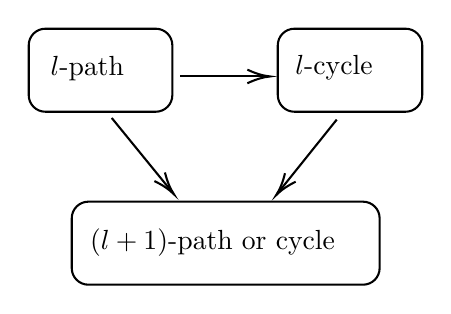
\begin{tikzpicture}[x=0.75pt,y=0.75pt,yscale=-1,xscale=1]
    % Rounded Rect [id:dp2247988663004169] 
    \draw   (100.6,84) .. controls (100.6,79.58) and (104.18,76) .. (108.6,76) -- (161.8,76) .. controls (166.22,76) and (169.8,79.58) .. (169.8,84) -- (169.8,108) .. controls (169.8,112.42) and (166.22,116) .. (161.8,116) -- (108.6,116) .. controls (104.18,116) and (100.6,112.42) .. (100.6,108) -- cycle ;
    % Rounded Rect [id:dp3322171879942837] 
    \draw   (220.6,84) .. controls (220.6,79.58) and (224.18,76) .. (228.6,76) -- (282.2,76) .. controls (286.62,76) and (290.2,79.58) .. (290.2,84) -- (290.2,108) .. controls (290.2,112.42) and (286.62,116) .. (282.2,116) -- (228.6,116) .. controls (224.18,116) and (220.6,112.42) .. (220.6,108) -- cycle ;
    % Rounded Rect [id:dp522325016929076] 
    \draw   (121.33,167.33) .. controls (121.33,162.92) and (124.92,159.33) .. (129.33,159.33) -- (261.67,159.33) .. controls (266.08,159.33) and (269.67,162.92) .. (269.67,167.33) -- (269.67,191.33) .. controls (269.67,195.75) and (266.08,199.33) .. (261.67,199.33) -- (129.33,199.33) .. controls (124.92,199.33) and (121.33,195.75) .. (121.33,191.33) -- cycle ;
    % Straight Lines [id:da4471732816066223] 
    \draw    (173.53,99) -- (214.87,99) ;
    \draw [shift={(216.87,99)}, rotate = 180] [color={rgb, 255:red, 0; green, 0; blue, 0 }  ][line width=0.75]    (10.93,-3.29) .. controls (6.95,-1.4) and (3.31,-0.3) .. (0,0) .. controls (3.31,0.3) and (6.95,1.4) .. (10.93,3.29)   ;
    % Straight Lines [id:da08077221270601986] 
    \draw    (140.6,119) -- (169.34,154.25) ;
    \draw [shift={(170.6,155.8)}, rotate = 230.81] [color={rgb, 255:red, 0; green, 0; blue, 0 }  ][line width=0.75]    (10.93,-3.29) .. controls (6.95,-1.4) and (3.31,-0.3) .. (0,0) .. controls (3.31,0.3) and (6.95,1.4) .. (10.93,3.29)   ;
    % Straight Lines [id:da17940502186011487] 
    \draw    (249,119.8) -- (221.05,154.64) ;
    \draw [shift={(219.8,156.2)}, rotate = 308.74] [color={rgb, 255:red, 0; green, 0; blue, 0 }  ][line width=0.75]    (10.93,-3.29) .. controls (6.95,-1.4) and (3.31,-0.3) .. (0,0) .. controls (3.31,0.3) and (6.95,1.4) .. (10.93,3.29)   ;

    % Text Nodes
    \draw (109.6,87.67) node [anchor=north west][inner sep=0.75pt]   [align=left] {$l$-path};
    \draw (227.6,87.27) node [anchor=north west][inner sep=0.75pt]   [align=left] {$l$-cycle};
    \draw (128.67,171) node [anchor=north west][inner sep=0.75pt]   [align=left] {$(l+1)$-path or cycle};
    \end{tikzpicture}
\end{center}

The algorithm considers two primary cases: when the object is a path and when it is a cycle.

\section{Path of Length $l$}

In this case, we start with a path \( P = \{x_1, e_1, \dots, x_{l}, e_{l}, x_{l + 1}\} \) of length \( l \). The goal is to find either a path of length \( l+1 \) or a cycle of length \( l \) or \( l+1 \). To assist in this process, we define the following variables:

\begin{itemize}
    \item \texttt{colors\_in\_path}: An array of size \( n \) where \texttt{colors\_in\_path[i]} is \texttt{True} if color \( i \) is used in the edges of the path.
    \item \texttt{vertices\_in\_path}: An array of size \( n \) where \texttt{vertices\_in\_path[i]} is \texttt{True} if vertex \( i \) is included in the path.
\end{itemize}

Let's divide the proof into two cases: when \( l \geq \left \lceil \frac{n}{2} \right \rceil \) and when \( l < \left \lceil \frac{n}{2} \right \rceil \).

\subsection{Case 1: \( l < \left \lceil \frac{n}{2} \right \rceil \)}

In this case, we select a color \( c \) that is not present among the edges of the current path. Since \( \deg(x_{l + 1}, c) \geq \left \lceil \frac{n}{2} \right \rceil \), and there are at most \( l < \left \lceil \frac{n}{2} \right \rceil \) vertices in the path, there must be a vertex \( y \) outside the path that is adjacent to \( x_{l + 1} \) via an edge in \( E(G_c) \). This guarantees that we can extend the path or create a cycle.

\begin{algorithm}
    \caption{Path Extension for \( l < \left \lceil \frac{n}{2} \right \rceil \)}
    \begin{algorithmic}[1]
        \Function{Extend\_Path\_Small}{$G, P$}
        \State \textbf{assert} \( P.\text{size()} < \lceil \frac{n}{2} \rceil \)
        \State $vertices \gets P.\text{vertices}$
        \State $edges \gets P.\text{edges}$
        \State $last\_vertex \gets P.\text{back()}$
        \For{$color \in \{0, \dots, n-1\}$}
            \If{\textbf{not} $colors\_in\_path[color]$} \Comment{Search for an unused color}
                \For{$i \in \{0, \dots, n-1\}$}
                    \If{\textbf{not} $vertices\_in\_path[i]$} \Comment{Check vertices outside the path}
                        \State $edge \gets G.\text{check\_edge}(last\_vertex, i, color)$
                        \If{$edge \neq \text{None}$}
                            \State $vertices.\text{append}(i)$
                            \State $edges.\text{append}(edge)$
                            \State \Return Path($G$, $vertices$, $edges$) \Comment{Return extended path}
                        \EndIf
                    \EndIf
                \EndFor
            \EndIf
        \EndFor
        \State \textbf{assert False, "No valid extension found"}
    \EndFunction
    \end{algorithmic}
\end{algorithm}

The time complexity of this function is \( O(n) \). Since we only need to find a color that is not in the path’s colors (which takes \( O(n) \)), and then locate a vertex outside the path that connects to the last vertex (also \( O(n) \)), the overall complexity remains linear in \( n \).

\section{Cycle of length $n - 1 \neq \ell \geq \left \lfloor \frac{n}{2} \right \rfloor$}

\section{Cycle of length $n - 1$}


